\documentclass[UTF8]{ctexart}
\usepackage{amsmath}
\usepackage{geometry}
\usepackage{graphicx}
\usepackage{gensymb}
\usepackage{wrapfig}
\usepackage{titlesec}
\usepackage{float}
\geometry{a4paper,scale=0.8}
\title{2017年媒体与认知期末试题答案}
\author{Deschain}
\titlespacing*{\section}
{0pt}{0pt}{0pt}
\titlespacing*{\subsection}
{0pt}{0pt}{0pt}
\titlespacing*{\paragraph}
{0pt}{0pt}{0pt}
\titlespacing*{\subparagraph}
{0pt}{0pt}{0pt}
\begin{document}
\maketitle
\section{填空题}
请务必将答案写到答题卡上,注明每一道题的题号。
\subsection{}
媒体是信息的\underline{载体}。
\subsection{}
信息,是物质相互作用中反映出的\underline{事物属性与状态}。
\subsection{}
认知,是指人认识客观世界事物的过程,是对作用于人的感觉器官的客观世界事物进行\underline{加工和处理}的过程。
\subsection{}
刚刚能引起差别感觉的刺激物间的最小差异量,称为\underline{阈值}。
\subsection{}
小波母函数为$\psi(t)$,尺度因子为a,$(a>0)$,平移因子为b,$(b\in R)$,则小波基函数为\underline{$\psi(\frac{t-b}{a})$}
\subsection{}
知觉的信息加工过程可以大致分为\underline{自下而上加工}和\underline{自上而下加工}。
\subsection{}
神经网络的学习过程主要由正向传播和\underline{反向传播}两个阶段组成。
\section{简答题}
\subsection{}
简述选择性注意的理论模型。
\paragraph{}
(1)过滤器模型:来自外界的信息是大量的,而人的神经系统高级中枢的加工能力是有限的。为避免系统超载,需要某种过滤器进行调节,选择其中较少的信息,使其进入高级分析阶段。这类信息受到进一步加工而被识别和存储,其他信息则不让通过。\\
(2)衰减模型(中期选择模型):高级分析水平的容量有限,必须由过滤器加以调节。过滤器允许一个通道的信息通过,也允许另一个通道的信息在受到衰减、强度减弱后通过,但其中一些信息仍可得到高级加工。\\
(3)反应选择模型:几个输入通道的信息均可以进入高级分析水平,得到全部的知觉加工。注意不在于选择知觉刺激,而在于选择对刺激的反应,即输出是按其重要性安排的,这种安排依赖于长期的倾向、上下文和指导语。感觉登记—知觉分析—反应选择—组织输出。
\subsection{}
简述人工神经元模型并画出结构图。
\paragraph{}
人工神经元包括两个计算步骤:
(1)线性加权求和,相当于两个向量$\vec x, \vec w$求内积。$z=\vec w^T\vec x$。式中$\vec x=(x_0,x_1,\cdots,x_d)^T$为输入数据$(x_1,\cdots,x_d)$的增广向量,$x_0=1$。$\vec w=(w_0,w_1,\cdots,w_d)^T$为权值向量,$w_0=b$为偏置量。
(2)激活函数:对数据进行非线性变换。$y=f(z)$。
\begin{figure}[H]
\centering
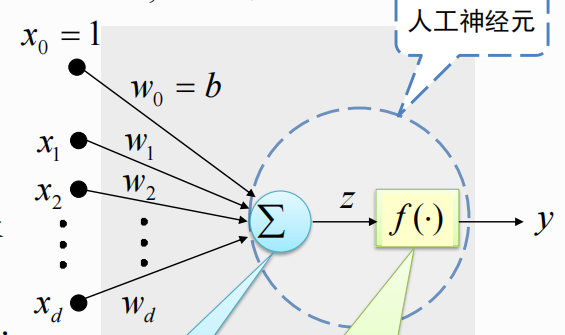
\includegraphics[width=3cm,height=3cm]{2017-1.png}
\end{figure}
\subsection{}
简述简单细胞对视觉刺激模式呈方向、位置、空间频率选择性的基本原理。
\paragraph{}
对大面积弥散光刺激没有反应,而对有一定方向或朝向的条纹刺激有强烈反应。若该刺激物的方向偏离该细胞“偏爱”的最优方位,则细胞反应停止或骤减。同时,它们对该类视觉刺激的位置和空间频率也表现出了明显的选择性。排成一条线的同心圆感受野聚合成一个简单感受野,从而对一定朝向的条形物敏感。
\subsection{}
请写出至少三种深度学习中防止过拟合的方法。
\paragraph{}
dropout、提前停止、$L_1$或$L_2$正则化、权值衰减、数据增强。
\section{计算题}
\subsection{}
设有两类正态分布的样本集,第一类均值为$\mu_1=(0.1,0.1)^T$,第二类均值为$\mu_2=(-1.5,2.0)^T$,方差$\sigma_1=\sigma_2=\begin{bmatrix}
1.2&0.4\\0.4&1.8\end{bmatrix}$,先验概率$p(\omega_1)=p(\omega_2)$。
(1)试求基于最小错误率的贝叶斯决策分界面。
\begin{equation*}
\begin{aligned}
&g_i(x)=-0.5(\vec x-\vec\mu)^T\sigma_i^{-1}(\vec x-\vec\mu)-0.5dln(2\pi)-0.5ln(\lvert\sigma_i\rvert)+ln(p(\omega_i))\\
&g_1(x)=-0.45x^2+0.07x+0.2xy+0.04y-0.3y^2-0.0055\\
&g_2(x)=-0.45x^2-1.75x+0.2xy+1.5y-0.3y^2-2.8125\\
g(x)=g_1(x)-g_2(x)=1.82x-1.46y+2.807
\end{aligned}
\end{equation*}
(2)根据最小错误率的贝叶斯分类器对特征向量 $x=(−0.5,1.0)^T$ 进行分类。
\[g(x)=0.437>0\]
属于第一类
\subsection{}
考虑一个两位寄存器。该寄存器具有四种可能的状态:00,01,10,11。在 t = 0 时,寄存器的内容随机算则为这四种状态之一,每种状态概率相同。在$t=n(n=1,2,3,\cdots)$时,寄存器随机操作如下:
按 1/6 的概率,保持不变;
按 1/2 的概率,寄存器的两位互换(例如,01 变为 10);
按 1/3 的概率,右边的一位翻转(例如,01 变为 00)。
寄存器以这种方式进行操作,左边的一位是观察值。
(1)用隐含马尔可夫模型对上述过程进行建模,写出状态转移概率矩阵。
\begin{equation*}
\begin{bmatrix}
\frac{2}{3} &\frac{1}{3} &0 &0\\
\frac{1}{3} &\frac{1}{6} &\frac{1}{2} &0\\
0 &\frac{1}{2} &\frac{1}{6} &\frac{1}{3}\\
0 &0 &\frac{1}{3} &\frac{2}{3}\\
\end{bmatrix}
\end{equation*}
(2)假设在 t = 1.1, 2.1, 3.1 时刻,我们观察到左边的一位为 1,1,0。请分析在 t = 1.1, 2.1, 3.1 时刻,
寄存器最可能的状态序列。
\begin{equation*}
\begin{aligned}
&\delta_1(1)=0\\
&\delta_1(2)=0\\
&\delta_1(3)=\frac{1}{4}\\
&\delta_1(4)=\frac{1}{4}\\
&\delta_2(1)=0\\
&\delta_2(2)=0\\
&\delta_2(3)=max\{0,\frac{1}{24},\frac{1}{12}\}\times1=\frac{1}{12}\\
&\varphi_2(3)=S_4\\
&\delta_2(4)=max\{0,\frac{1}{12},\frac{1}{6}\}\times1=\frac{1}{6}\\
&\varphi_2(4)=S_4\\
&\delta_3(1)=0\\
&\delta_3(2)=max\{0,0,\frac{1}{24}\}\times1=\frac{1}{24}\\
&\varphi_3(4)=S_4S_3\\
&\delta_3(3)=0\\
&\delta_3(4)=0\\
\end{aligned}
\end{equation*}
最有可能是$S_4S_3S_2$
\subsection{}
给定八个训练样本,正样本为$D_1=(0,3)^T,D_2=(3,0)^T,D_3=(0,-3)^T,D_4(-2,0)^T$,负样本为$D_5(1,1)^T,D_6=(0.5,-1)^T,D_7=(-1,-1)^T,D_8=(-1,0.5)^T$。请采用非线性支持向量机设计分类器。
(1)请选择一个合适的核函数,画出基于该核函数支持向量机的分类界面示意图,并通过观察法写出支持向量。
画图略。
支持向量为(-1,-1),(1,1),(-2,0)。
(2)请写出分类界面函数。
\begin{equation*}
g(x,y)=x^2+y^2-3
\end{equation*}
\subsection{}
假设如下左图是二维卷积神经网络某层某通道的特征图,如下右图为下一层的一个 3 × 3 卷积核:
\begin{figure}[H]
\centering
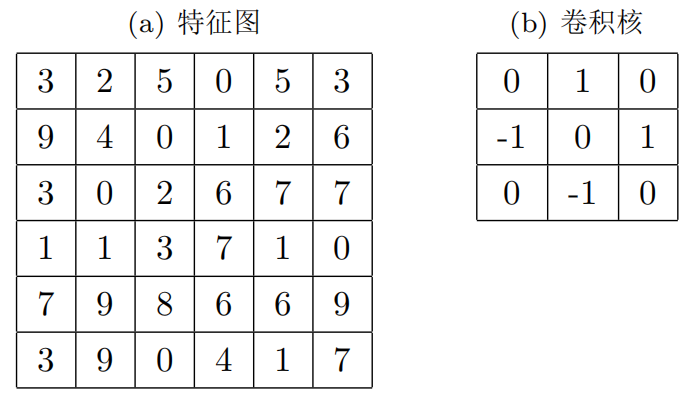
\includegraphics[width=6cm,height=4cm]{2017-2.png}
\end{figure}
(1)卷积操作是卷积神经网络的必要步骤。请写出上述卷积核滤波后的特征图,其中边界延拓(padding)参数为 0,卷积步长(stride)参数为 1。 
\begin{equation*}
\begin{bmatrix}
-1&0&-4&3\\
2&3&-1&1\\
-7&0&-2&-6\\
-7&0&1&3
\end{bmatrix}
\end{equation*}
(2)请写出卷积之后的特征图再经过一个最大值池化(max-pooling)层之后的特征图,其中 kernel 大小为 2 ,stride 参数为 2 。
\begin{equation*}
\begin{bmatrix}
3&3\\
0&3
\end{bmatrix}
\end{equation*} 
(3)请写出(a)中卷积核滤波后的特征图以 ReLU 函数为激活函数的输出特征图。
\begin{equation*}
\begin{bmatrix}
0&0&0&3\\
2&3&0&1\\
0&0&0&0\\
0&0&1&3
\end{bmatrix}
\end{equation*}
\end{document}